\documentclass[a4paper,10pt]{article}
\usepackage{src/preamble}
\usepackage[
	backend=biber,
	maxalphanames=10,
]{biblatex}
\bibliography{accelerator.bib}


\begin{document}

\noindent
\begin{center}
	\textbf{{\Large RELAZIONE ACCELERATORE - IL CICLOTRONE}} \\
\end{center}

\noindent
\textbf{Autore: Alessandro Biagiotti} \hfill \textit{Università degli studi di Milano, Milano,
	Italia}
\\

\phantomsection
\makeatletter\def\@currentlabel{\texttt{(I)}}\makeatother
\label{sec:intro}
\noindent
\textbf{INTRODUZIONE:}
\\
Il ciclotrone fu il primo acceleratore ciclico inventato da Ernest Lawrence nel 1929-1930 e
successivamente patentato nel 1932, un esempio della struttura dell'acceleratore può essere vista
in Figura \ref{fig:cyclotron}. La particella, partendo da una posizione centrale, esegue un
moto spiraliforme verso l'esterno dell'acceleratore (aumentando quindi il raggio di curvatura a ogni
giro). L'acceleratore è costituito da due diverse \emph{dee}, un generatore a corrente alternata dà
un \emph{kick} alla particella ogni volta che questa si trova nel territorio di collegamento tra le
due dee. La dee all'interno della quale viaggia la particella non è altro che un conduttore che ha
le proprietà di un \emph{drift}.

\begin{figure}[h!]
	\centering

	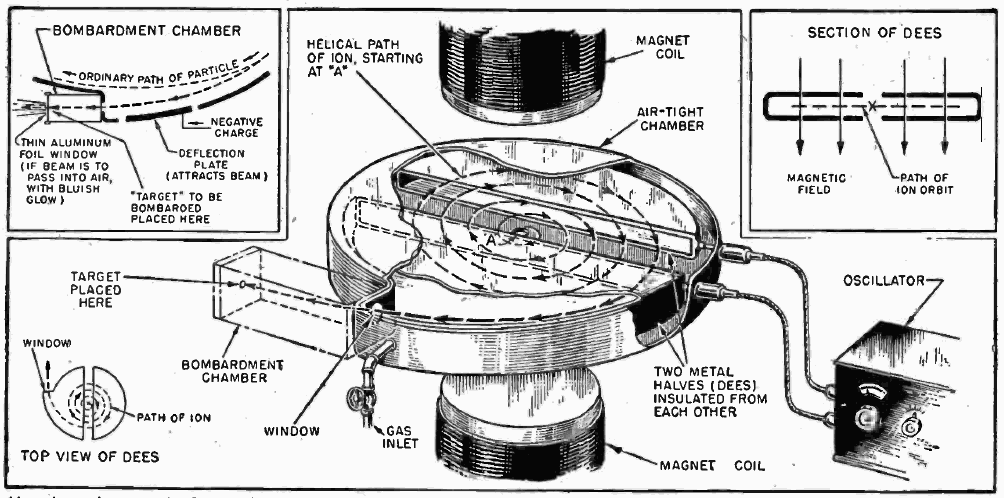
\includegraphics[scale=0.35]{fig/Cyclotron-diagram.png}
	\caption{
		La struttura di un ciclotrone
	}\label{fig:cyclotron}
\end{figure}

\bigskip
\phantomsection
\makeatletter\def\@currentlabel{\texttt{(II)}}\makeatother
\label{sec:cyclotron}
\noindent
\textbf{LA FISICA DEL CICLOTRONE:}

\clearpage

\printbibliography

\end{document}
